\begin{figure}[!h]
  \begin{subfigure}{.5\textwidth}
    \centering
    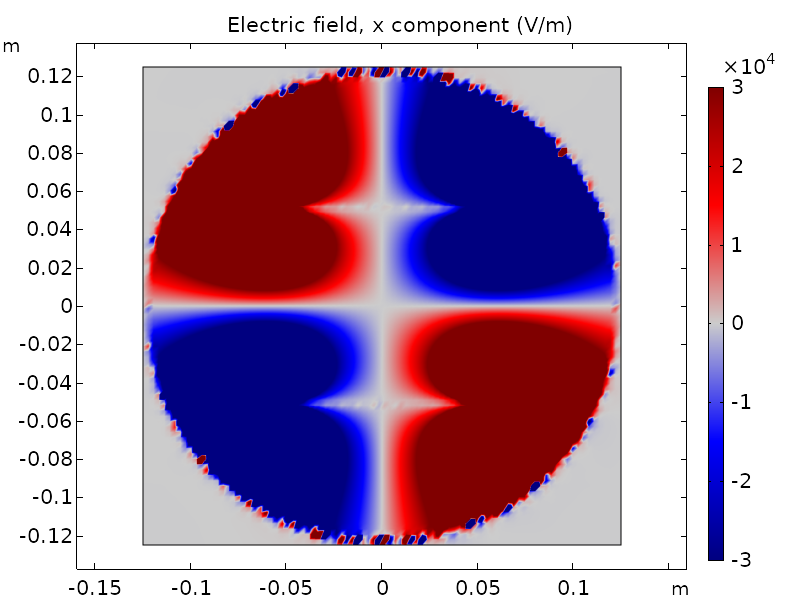
\includegraphics[width=\textwidth]{03_Prototype/figures/fig012_BEMa.png}
    \caption{Configuration 1 solved with BEM.}
    \label{}
  \end{subfigure}\hfill
  \begin{subfigure}{.5\textwidth}
    \centering
    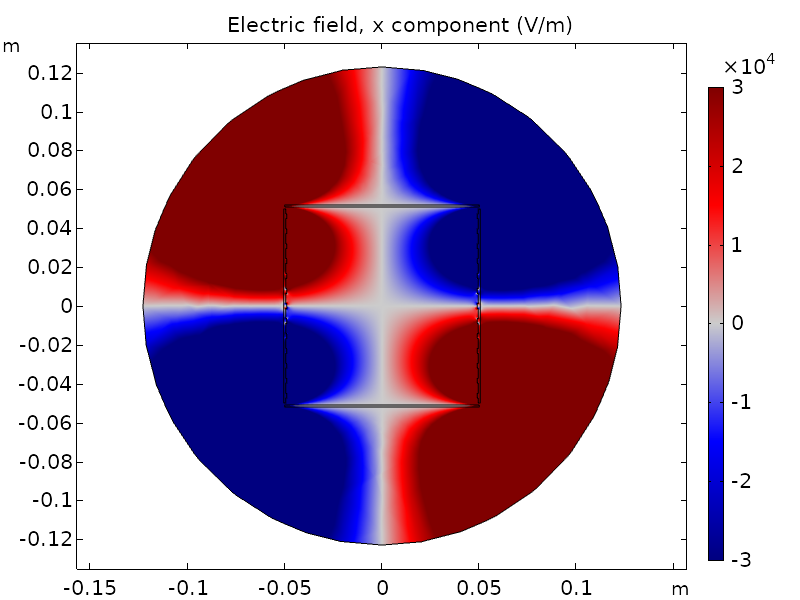
\includegraphics[width=\textwidth]{03_Prototype/figures/fig012_FEMa.png}
    \caption{Configuration 1 solved with FEM.}
    \label{}
  \end{subfigure}
  \vskip\baselineskip
  \begin{subfigure}{.5\textwidth}
    \centering
    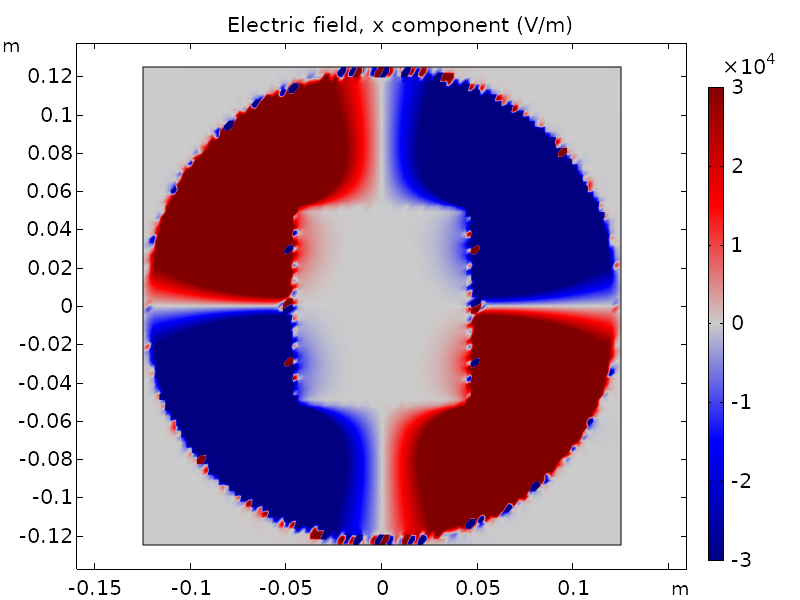
\includegraphics[width=\textwidth]{03_Prototype/figures/fig012_BEMb.png}
    \caption{Configuration 2 solved with BEM.}
    \label{}
  \end{subfigure}\hfill
  \begin{subfigure}{.5\textwidth}
    \centering
    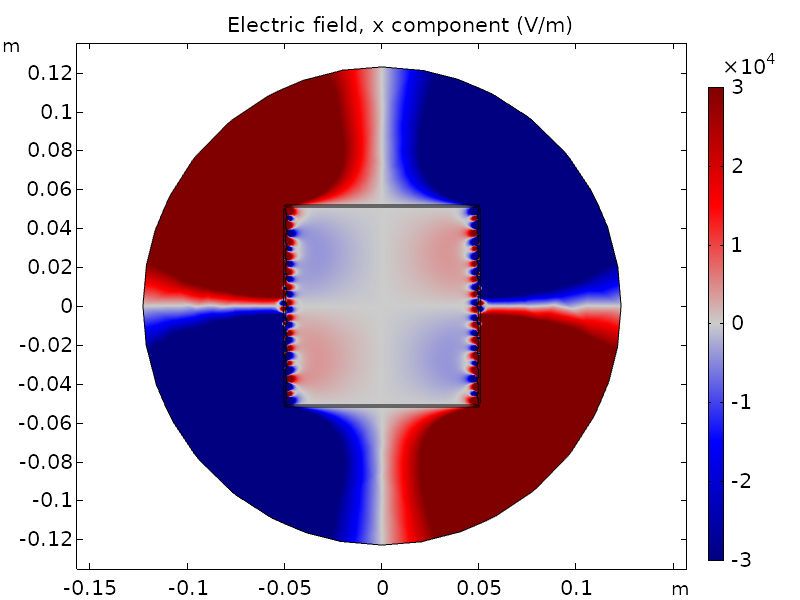
\includegraphics[width=\textwidth]{03_Prototype/figures/fig012_FEMb.png}
    \caption{Configuration 2 solved with FEM.}
    \label{}
  \end{subfigure}
  \caption[Comparison beetwen BEM and FEM for two different IPM configurations]{Comparison beetwen BEM and FEM for two different IPM configurations.}
  \label{chap3:FEMvsBEM}
\end{figure}
